\documentclass{beamer}
\renewcommand\thesection{\arabic{section}}
\newcommand{\myfont}{\rmfamily\normalsize\upshape\mdseries}
\newcommand{\degree}{^\circ}
\newcommand{\R}{\mathbb{R}}
\newcommand{\h}{\hspace{1em}}
\newcommand{\vs}{\vspace{1em}}
\title{\sffamily Final RC Part II}
\subtitle{\textbf{Practical Integral}\\}
\institute[UM-SJTU JI]{University of Michigan-Shanghai Jiao Tong University Joint Institute}
\author{HamHam}
\usepackage{graphicx}
\usepackage{picinpar}
\usepackage{indentfirst}
\usepackage{chemformula}
\usepackage{geometry}
\usepackage{subfigure}
\usepackage{appendix}
\usepackage{amsfonts,amsmath,amssymb}
\usepackage{enumerate}
\usepackage{float}
\usepackage{geometry}
\usepackage{latexsym}
\usepackage{listings}
\usepackage{multicol,multirow,multido}
\usepackage{tabularx}
\usepackage{ulem}
\usepackage{tikz}
\usepackage{xcolor}
\usepackage{cite}
\usepackage{setspace}
\usepackage{hyperref}
\usepackage{textpos}
\usepackage{booktabs}

\usetheme[dove]{Boadilla}
\usecolortheme{dolphin}
\useoutertheme{miniframes}
\begin{document}
    \usebackgroundtemplate{\tikz\node[opacity=0.3]{
    
\includegraphics[width=\paperwidth,
    height=\paperheight]{hamster.jpg}
    };}
\begin{titlepage}
    \begin{center}
        VV186 - Honors Mathmatics II
    \end{center}
\end{titlepage}
\myfont
\begin{frame}
    \frametitle{Integration Method}
    \begin{itemize}
        \item Recite the table
        \item Substitution (using trigonometric functions)
        \item Integration by parts + DI table
        \item Pay attention to the range
        \item Some Trick: Symmetry
    \end{itemize}
    \vspace{1em}
    \hspace{1em} Exercises: For $a>0$, calculte 
    $$\int_{-a}^a \frac{\cos(x)}{1+e(x)^{o(x)}} dx$$
    where $e(x)$ is a continuous strictly positive even function, and $o(x)$ is an odd function
\end{frame}
\begin{frame}
    \frametitle{Fundamental Theorem of Calculus}
    Let $f ~: [a, b] \to \mathbb{C}$ be continuous and set
    $$F : [a, b] \to \mathbb{C} ~~~~~~~~F(x) := \int_a^x f.$$
    Then F is differentiable on $(a, b)$ and
    $$F~'(x) = f ~(x), ~~~~~~~~~x \in (a, b)$$
\end{frame}
\begin{frame}
    \frametitle{Question on Piazza}
    \centering
    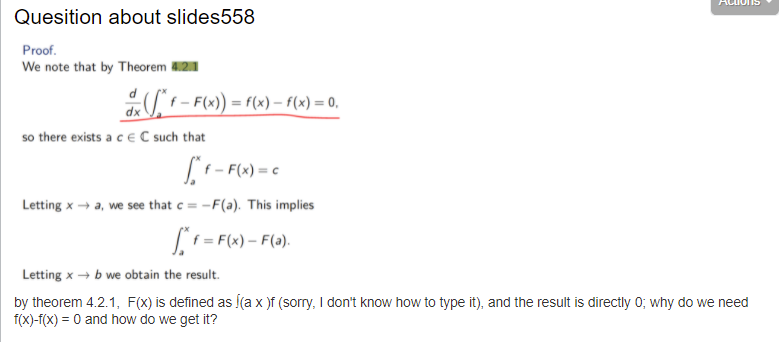
\includegraphics[height=0.4\textwidth]{question.png}
    \begin{block}{A class of functions}
        Instead, the $F(x)$ that we are discussing here is about the primitive, 
        namely, $F(x)$ could be any function that satisfies $F~'(x) = f~(x)$.
    \end{block}
\end{frame}
\begin{frame}
    \frametitle{Exercise}
    Calculate:
    $$\underset{x\to 0}{\lim}\frac{\int_0^{x^2} \ln (1+t)dt}{(e^{x^2}-1)\sin ^2 x}$$
    \pause
    \centering
    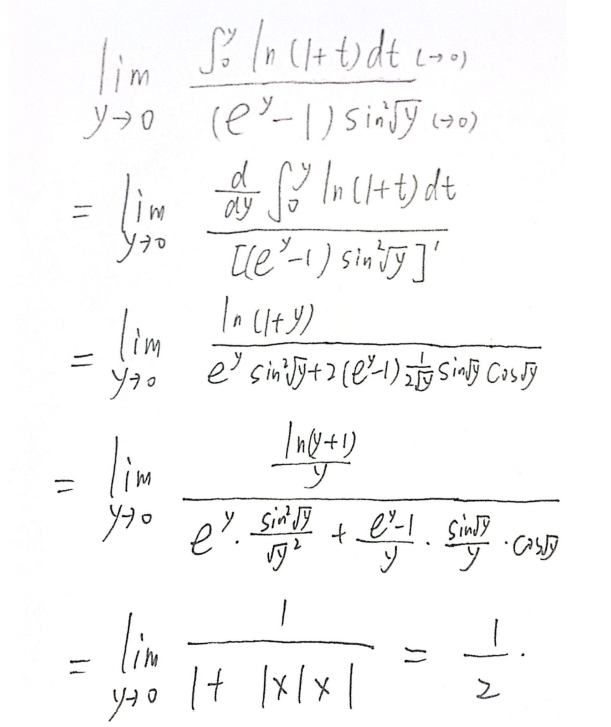
\includegraphics[height=0.6\textheight]{solution.png}
\end{frame}
\begin{frame}
    \frametitle{Improper Integral}
    An integral $$\int_a^b f(t)dt$$ is called improper if
    \begin{itemize}
        \item the domain of integration is unbounded. i.e. $a=-\infty$
        \item the integrand f is unbounded on $(a, b)$ or otherwise not regulated
    \end{itemize}

\end{frame}
\begin{frame}
    \frametitle{Calculation of improper integral}

    \hspace{1em}
Let's just assume that they all exist. The convergence theorem
will be talked about later.\\
\vspace{1em}
\textcolor{red}{Method1: calculate just like normal integral.}
$$\int_1^\infty \frac{dx}{e^{x+1}+e^{3-x}}$$
\pause
\begin{align*}
    &\int_1^\infty \frac{dx}{e^{x+1}+e^{3-x}}=\frac{1}{e}\int_1^\infty \frac{d e^x }{e^{2x}+e^2}\\
    \xrightarrow{t=e^x}&=\frac{1}{e}\int_0^\infty \frac{dt}{t^2+e^2}=\frac{1}{e^2} \arctan \frac{t}{e} \bigg|_0^\infty=\frac{\pi}{2e^2}
\end{align*}
\end{frame}
\begin{frame}
    \frametitle{Calculation of improper integral}
    \textcolor{red}{Method2: Symmetry}
    \begin{itemize}
        \item $$\int_0^\infty \frac{\ln x}{1+x^2}$$
        \item $$\int_0^\frac{\pi}{2} \ln \sin (x) dx$$
    \end{itemize}
\end{frame}

\begin{frame}
    \frametitle{Convergence?}
    Cauchy Criterion:\\
    \hspace{1em}
    Let $a\in \mathbb{R} $ and $f:[a,\infty) \to \mathbb{R}$ be integrable
    on every interval $[a,x],x \in \R$. The improper integral
    $$\int_a^\infty f~(x ) dx $$
    converges if and only if 
    $$\underset{\varepsilon>0}{\forall}~ \underset{R>0}{\exists} ~\underset{x,y>R}{\forall} ~|\int_x^y f~(t) dt| < \varepsilon$$
\end{frame}
\begin{frame}
    \frametitle{Comparison test}
    \h Let $I \subset \R$ and $f: I \to \mathbb{C}, g: I \to [0,\infty).$
Suppose that      $|f~(t)|\leq g(t)$ for $t \in I $ and $\int_I g(t)dt $ converges.
Then $\int_I f~(t)dt$ also converges.\\
    \vs \h
    Is it convergent?
    $$\int_1^{+\infty} \frac{\sin x}{x\sqrt{x}} dx$$
    \pause
    Since 
    $$|\frac{\sin x}{x\sqrt{x}}|\leq |\frac{1}{x\sqrt{x}}|=\frac{1}{x^{\frac{3}{2}}}$$ 
    it is convergent.
\end{frame}
\begin{frame}
    \frametitle{Absolute and Conditional Convergence}
    \h Let $I \subset \R$ and $f: I \to \mathbb{C}$. We say that the improper inteegral $\int_I f~(t)dt$
    \vs
    \begin{itemize}
        \item \textbf{\textcolor{blue}{converges absolutely}} if $\int_I |f~(t)| dt$ converges.
        \item if $\int_I f~(t) dt$ converges but $\int_I |f~(t)| dt$ not, it's \textbf{\textcolor{blue}{conditionally convergent}}.
    \end{itemize}
    \vs
    \begin{block}{Terrible Example}
        Analyse the convergence and absolute convergence of 
        $$\int_0^\infty [(1-\frac{\sin x}{x})^{-\frac{1}{3}}-1]dx$$
    \end{block}
\end{frame}
\begin{frame}
    \frametitle{Friendly Example¿}
    \begin{itemize}
        \item Though $\underset{n \to \infty}{\lim} \int_0^n \sin(2\pi x) =0$, the integral $\int_0^\infty \sin (2\pi x) $ doesn't exist 
        \item Let $f:[0, +\infty)\to \R$, $f(x)=\frac{e^x}{n!}$ when $x \in [n,n+1)$. The integral $\int_0^\infty f$ exists and converges absolutely. 
        \item \textcolor{red}{The integral $\int_0^\infty \sin x^2 $  exists and converges conditionally.} 
        \item The integral $\int_a^\infty \frac{\cos(x)}{x}$ is conditionally convergent for all $a>0$, and $\int_0^\infty  \frac{\cos(x)}{x}$ also exists 
        
    \end{itemize}
    

\end{frame}
\begin{frame}
    \frametitle{Euler Gamma Function}
     $$\Gamma : \R_+ \to \R, ~~~~~ \Gamma(t):=\int_0^\infty z^{t-1}e^{-z}dz,~~~~~ t>0$$
    Basic properties:
    \begin{itemize}
        \item For any $t>0$, we have $\Gamma(t+1)=t\Gamma(t)$
        \item For $n\in \mathbb{N}^*$, we have $\Gamma(n)=n!$
    \end{itemize}
    \vs
    Not so important now, but is really important in VE401.
\end{frame}
\begin{frame}
    \frametitle{Reference}
    \begin{itemize}
        \item Exercises from 2020--Vv186 TA-Zhang Chengsong.
        \item Exercises from 2019--Vv186 TA-Zhang Leyang
        \item Exercises from my RC8.
        \item Exercise from JI first integration bee.
    \end{itemize}
\end{frame}
\end{document}